\documentclass[aspectratio=149]{beamer}
% The values that it accepts are: 1610, 169, 149, 54, 43 and 32, which stand for the ratios 16:10, 16:9, 14:9, 5:4, 4:3 and 3:2, respectively.

% Idioma y codificacion en castellano
\usepackage[T1]{fontenc}
\usepackage[utf8]{inputenc}
\usepackage[english, spanish, es-tabla]{babel}

% Otros
\usepackage{fontspec}
\usepackage{unicode-math}
\usepackage{lmodern}
\usepackage{setspace}
\usepackage{csquotes}

% Imagenes
\usepackage{graphicx}
\graphicspath{{img/}}

% Bibliografía
\usepackage{biblatex}
\addbibresource{bibliografia.bib}

% Colores
\definecolor{link}{rgb}{0,0.4,0.6}
\definecolor{url}{rgb}{0.6,0,0}

% TODO list
\usepackage{pifont}
\usepackage{amssymb}

% Enlaces
\hypersetup{
    colorlinks = false,
    linktocpage = true,
    urlcolor = {url},
    linkcolor = {link},
    citecolor = {citation},
    pdfpagemode = {UseOutlines},
    pdfstartview = {Fit}}

% Titulo
\titlegraphic{
    \begin{center}
        
\includegraphics[height=2cm]{img/escudoUBU} \hspace{1cm}
        
\includegraphics[height=2cm]{img/escudoUVA} \hspace{1cm}
        
\includegraphics[height=2cm]{img/escudoULE} \vspace{1cm}
    \end{center}}

\setbeamertemplate{title page}{
    \begin{center}
        \vspace{0.4cm}
        {\textbf{\LARGE\inserttitle}}\\[0.8cm]
        \fontfamily{ptm}\selectfont
        {\insertauthor}\\[0.4cm]
        {\scriptsize\insertinstitute}\\[0.25cm]
        {\insertdate}\\[0.5cm]
        \inserttitlegraphic
    \end{center}}

%%% =========================
%%%  Nouveaux environnements
%%% =========================

%% Environnements pour les demo de code; tirés du document
%% principal. (L'environnement 'eqxample' ajoute des filets de part
%% et d'autre du bloc pour illustrer les marges.)
\newenvironment{demo}{%
    \begin{beamercolorbox}[wd=\linewidth,sep=6pt]{block body example}}
    {\end{beamercolorbox}}

\newenvironment{texample}[1][0.45\linewidth]{%
    \noindent\begin{minipage}{#1}%
    \def\producing{\end{minipage}\hfill\begin{minipage}{\dimexpr0.9\linewidth-#1}%
        \hbox\bgroup\kern-.2pt%
        \vbox\bgroup\parindent0pt\relax
        % The 3pt is to cancel the -\lineskip from \displ@y
        \abovedisplayskip3pt \abovedisplayshortskip\abovedisplayskip
        \belowdisplayskip0pt \belowdisplayshortskip\belowdisplayskip
        \noindent}
    }{%
        \par
        % Ensure that a lonely \[\] structure doesn't take up width less than
        % \hsize.
        \hrule height0pt width\hsize
        \egroup\kern-.2pt\egroup
        \end{minipage}%
        \par
    }

\newenvironment{eqxample}{%
    \noindent\begin{minipage}{.45\linewidth}%
    \def\producing{\end{minipage}\hfill\begin{minipage}{.45\linewidth}%
        \hbox\bgroup\kern-.2pt\vrule width.2pt%
        \vbox\bgroup\parindent0pt\relax
        % The 3pt is to cancel the -\lineskip from \displ@y
        \abovedisplayskip3pt \abovedisplayshortskip\abovedisplayskip
        \belowdisplayskip0pt \belowdisplayshortskip\belowdisplayskip
        \noindent}
    }{%
        \par
        % Ensure that a lonely \[\] structure doesn't take up width less than
        % \hsize.
        \hrule height0pt width\hsize
        \egroup\vrule width.2pt\kern-.2pt\egroup
        \end{minipage}%
        \par
  }

%% Simplfication de l'environnement 'quote' de beamer
\renewenvironment{quote}{%
    \begin{beamercolorbox}[wd=\linewidth,sep=6pt]{block body example}}
    {\end{beamercolorbox}}

%% Exercices
\newenvironment{exercice}{%
    \begin{frame}[fragile=singleslide]
    \frametitle{\faCogs\; Exercice}}{\end{frame}}
  
%%% =======
%%%  Varia
%%% =======

%% Longueurs pour la composition des pages couvertures avant et
%% arrière.
\newlength{\banderougewidth} \newlength{\banderougeheight}
\newlength{\bandeorwidth}    \newlength{\bandeorheight}
\newlength{\imageheight}
\newlength{\logoheight}

\mode<presentation> {
    \usetheme{ulaval}
    \setbeamercovered{transparent}
    \setbeamertemplate{navigation symbols}{}
}

\newenvironment{xframe}[2][]
    {\begin{frame}[fragile,environment=xframe,#1]
    \font
    \frametitle{#2}}
    {\end{frame}}

\AtBeginSection[]{
    \begin{frame}
    \huge \centerline{\insertsection}
    \small \tableofcontents[currentsection, hideothersubsections]
    \end{frame}
}

\setcounter{tocdepth}{2}
\newcommand{\acc}[1]{\textcolor{ulred}{\textbf{#1}}}


\title[Automatización del proceso de adquisición de imágenes de redes sociales para sistemas de recomendación]{Automatización del proceso de adquisición de imágenes de redes sociales para sistemas de recomendación}

\author[Daniel González Alonso]{
    Autor: Daniel González Alonso\\[1ex] 
    Tutor: Ángel Manuel Guerrero Higueras}
\institute[Universidad de Valladolid]
{
    Máster Universitario en Inteligencia de Negocio \\[-4pt]
    y Big Data en Entornos Seguros
	%\medskip
	%{\emph{daniel.gonzalez.alonso@alumnos.uva.es}}
}



\titlegraphic{%
    \begin{center}
        
\includegraphics[height=2cm]{img/escudoUBU} \hspace{1cm}
        
\includegraphics[height=2cm]{img/escudoUVA} \hspace{1cm}
        
\includegraphics[height=2cm]{img/escudoULE} \vspace{1cm}
    \end{center}}

\setbeamertemplate{title page}{%
    \begin{center}
        \vspace{0.4cm}
        {\textbf{\LARGE\inserttitle}}\\[0.8cm]
        \fontfamily{ptm}\selectfont
        {\insertauthor}\\[0.4cm]
        {\scriptsize\insertinstitute}\\[0.25cm]
        {\insertdate}\\[0.5cm]
        \inserttitlegraphic
    \end{center}}



\begin{document}

%==============================================================================
% Título
%==============================================================================
\begin{frame}[label=title, plain]
    \titlepage
\end{frame}

%==============================================================================
% TABLA DE CONTENIDOS
%==============================================================================
\begin{frame}[label=toc]{Tabla de contenidos}
 \setlength{\leftskip}{5cm}%
 \tableofcontents[subsectionstyle=hide]
\end{frame}

%==============================================================================
% INTRODUCCION
%==============================================================================
\section{Introducción}
\begin{frame}[label=intro]{Introducción}
    \begin{itemize}
        \item La monitorización y análisis de redes actualmente es un problema muy complejo debido a su tamaño y tráfico.
        \item Los métodos convencionales hacen uso de servidores centrales. Problemas:
        \begin{itemize}
            \item Limitaciones de cómputo
            \item Punto de fallo único.
        \end{itemize}
        \item Propuesta: Sistema de monitorización distribuido para el protocolo TCP empleando \textit{Spark Streaming}.
    \end{itemize}
\end{frame}

\begin{frame}[label=spark_streaming]{Spark Streaming}
    \begin{itemize}
        \item Hadoop es una plataforma que emplea un modelo MapReduce para procesar gran cantidad de datos.
        \item Para reducir el uso de la entrada/salida y con ello mejorar el rendimiento se creó Apache Spark.
        \item Ambas plataforma fueron ideadas para analizar grandes cantidades de datos en Batch mediante MapReduce.
        \item En la actualidad Spark ofrece la librería \textbf{Spark Streaming} para poder usarlo con streams de datos empleando una técnica conocida como \textit{micro-batching}.
    \end{itemize}
\end{frame}

%==============================================================================
% OBJETIVOS
%==============================================================================
\section{Objetivos}
\begin{frame}[label=objetivos]{Objetivos}
    \begin{itemize}
        \item \textbf{Objetivos generales}: conocer el estado del arte, desarrollar el software necesario para la descarga de publicaciones, análisis de emoción sobre las publicaciones, hacer una visualización.
        \item \textbf{Objetivos técnicos}: uso de herramientas en la nube para el alojamiento y procesamiento de datos, el proyecto no ha de suponer ningún coste, crear un cuadro de mandos para la visualización.
        \item \textbf{Objetivos personales}: aprender a usar herramientas y servicios en la nube, mejorar mis conocimientos sobre almacenamiento y procesado de grandes cantidades de datos, poner en práctica mis conocimientos sobre cuadros de mando.
    \end{itemize}
\end{frame}

%==============================================================================
% TRABAJOS RELACIONADOS
%==============================================================================
\section{Trabajos Relacionados}
\begin{frame}[label=relat]{Trabajos Relacionados}
    \begin{itemize}
        \item Sistema BRO para detectar intrusos en redes mediante un motor de eventos, el cual podía customizarse empleando un lenguage de scripting. Problema: un solo hilo.
        \item Gupta et al. propusieron un sistema para analizar redes en tiempo real mediante \textit{Spark Streaming}. Problema: solo funcionan mediante switchs programables.
        \item Karimi et al. propusieron un sistema distribuido de análisis de tráfico que captura paquetes y guarda sus cabeceras en un CSV que se procesa periódicamente. Problema: el rendimiento puede degradarse.
    \end{itemize}
\end{frame}

%==============================================================================
% TECNICAS Y HERRAMIENTAS
%==============================================================================
\section{Técnicas y Herramientas}
\begin{frame}[label=herramientas]{Técnicas y Herramientas}
    \begin{itemize}
        \item \textbf{Instalooter}
        \item Servicios en la nube con \textbf{Amazon Web Services}:
        \begin{itemize}
            \item Rekognition
            \item Amazon S3
            \item Amazon EC2
            \item DynamoDB
            \item AWS Lambda
            \item Amazon API Gateway
        \end{itemize}
        \item \textbf{Grafana}
        \item Otras herramientas:
        \begin{itemize}
            \item \texttt{virtualenv}
            \item Visual Studio Code
            \item Git y GitHub
            \item \LaTeX y Overleaf
        \end{itemize}
    \end{itemize}
\end{frame}

%==============================================================================
% ASPECTOS RELEVANTES DEL DESARROLLO DEL PROYECTO
%==============================================================================
\section{Aspectos relevantes del desarrollo del proyecto}

\subsection{Métricas}
\begin{frame}[label=metricas]{Métricas}
    \begin{itemize}
        \item Throughput: número y longitud de los segmentos TCP por segundo.
        \item Ratio de retransmisón y out-of-order: Indica el ratio de mensajes que han llegado desordenados o que han sido retransmitidos. Si este ratio es malo, es un síntoma de mal rendimiento en la red.
        \item RTT: es el tiempo que tarda la comunicación en viajar desde el origen al destino y su correspondiente respuesta ACK.
    \end{itemize}
\end{frame}

\subsection{Sistema Propuesto}
\begin{frame}[label=sistema]{Sistema Propuesto}
    \begin{enumerate}
        \item Preprocesamiento: Los Collectors capturan segmentos TCP de la red y almacenan de cada uno una tupla, generando el stream \texttt{DStream0}. Este después es preprocesado para generar nuevas tuplas que añaden el siguiente número de secuencia esperado, creando otro stream \texttt{DStream1}.
        \item Cálculo de Throughput: de cada tupla de \texttt{DStream1} se calcula el número total de paquetes obtenidos entre un origen y un destino y la longitud total de los paquetes mediante \texttt{reduceByKey}. Esta información es almacenada en un nuevo stream \texttt{DStream2}.
    \end{enumerate}
\end{frame}
\begin{frame}{Sistema Propuesto}
    \begin{enumerate}
        \setcounter{enumi}{2}
        \item Retransmisión y out-of-order: A partir de \texttt{DStream1} se calcula el número de retransmisiones y de elementos desordenados mediante el siguiente algoritmo. El resultado se guarda en el stream \texttt{DStream3}.
        \begin{columns}
        \begin{column}{0.4\textwidth}
        	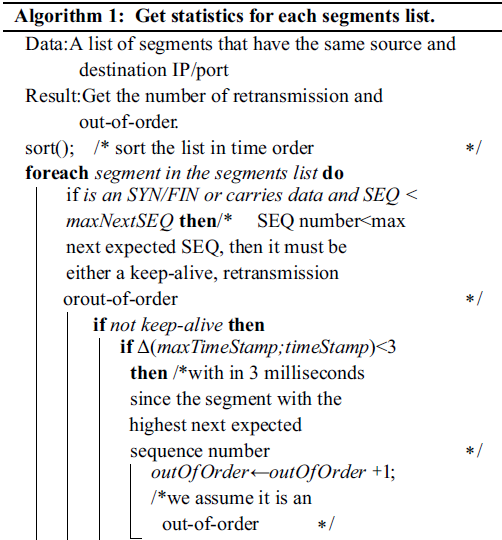
\includegraphics[width=1.0\textwidth]{img/alg1_1.png}
        \end{column}
        \begin{column}{0.4\textwidth}
        	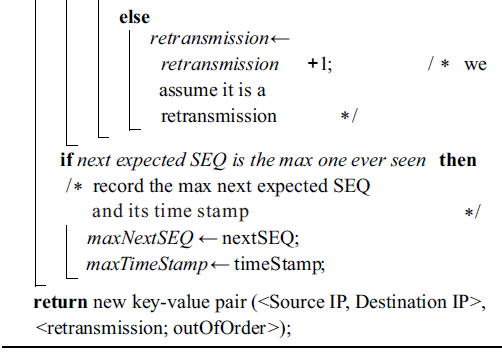
\includegraphics[width=1.0\textwidth]{img/alg1_2.png}
        \end{column}
        \end{columns}
    \end{enumerate}
\end{frame}
\begin{frame}{Sistema Propuesto}
    \begin{columns}
    \begin{column}{0.6\textwidth}
        \begin{enumerate}
            \setcounter{enumi}{3}
            \item RTT: los segmentos TCP y los segmentos ACK se agrupan mediante \texttt{groupByKey}, lo que permite calcular el RTT mediante el siguiente algoritmo. El resultado obtenido se almacena en el stream \texttt{DStream4}.
            \item Etapa final: se unen los datos obtenidos en el \texttt{DStream2}, \texttt{DStream3} y \texttt{DStream4} mediante una operación de \texttt{join} para poder mostrar los resultados al usuario.
        \end{enumerate}
    \end{column}
    \begin{column}{0.5\textwidth}
        \begin{figure}
            \centering
            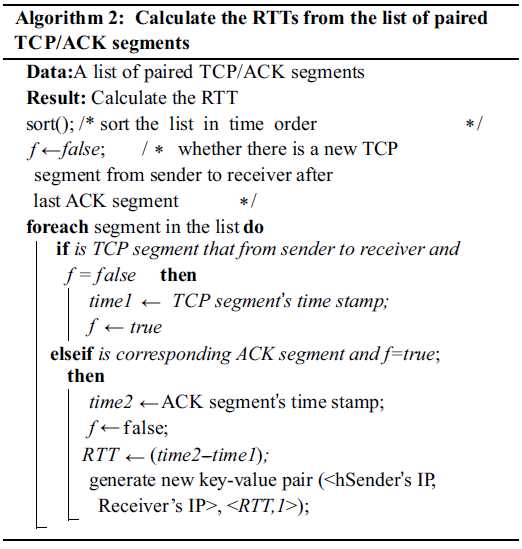
\includegraphics[width=1.0\textwidth]{img/alg2.png}
            %\caption{Algoritmo RTT}
            \label{fig:alg2}
        \end{figure}
    \end{column}
    \end{columns}
\end{frame}

%==============================================================================
% CONCLUSIONES Y LINEAS DE TRABAJO FUTURAS
%==============================================================================
\section{Conclusiones y Líneas de trabajo futuras}

\subsection{Conclusiones}
\begin{frame}[label=conclu]{Conclusiones}
    \begin{itemize}
        \item Se considera que se ha conseguido cumplir los objetivos generales inicialmente planteados.
        \item La base base de datos final ha estado más limitada de lo esperado.
        \item Los crawlers son muy sensibles a las actualizaciones de las páginas web.
        \item Usar DynamoDB presenta algunas limitaciones, tanto por las consultas que se pueden hacer como por el soporte de otras herramientas para conectarse a esta base de datos.
    \end{itemize}
\end{frame}

\subsection{Líneas de trabajo futuras}
\begin{frame}[label=lineas]{Líneas de trabajo futuras}
    \begin{itemize}
        \item Agrandar la base de datos.
        \item Ejecutar descarga de datos periódicamente de forma automática, ya sea mediante un cron o en AWS Lambda.
        \item Explotar el texto de la descripción de las publicaciones.
        \item Desarrollar una aplicación o una página web que sea más \textit{user friendly} en vez de usar un cuadro de mandos.
    \end{itemize}
\end{frame}

%==============================================================================
% Bibliografía
%==============================================================================
\begin{frame}{Bibliografía}
    \printbibliography
\end{frame}

\end{document}